\documentclass[conference]{IEEEtran}
\usepackage{amsmath}
\usepackage{amssymb}
\usepackage{graphicx}
\usepackage{booktabs}
\usepackage{url}
\usepackage[hidelinks]{hyperref}

\begin{document}

\title{Neural Q-Function Approximation for an Episodic\\ Stochastic Shortest-Path Problem}

\author{
\IEEEauthorblockN{Chinmay Prashanth, Arjun Singh Yadav, Mohammad Ibraheem}
\IEEEauthorblockA{Team 9 \\
EEE598, Arizona State University \\
cprashan@asu.edu, asyadav6@asu.edu, Mibrahe5@asu.edu}
}

\maketitle

\begin{abstract}
We replace the tabular Q-table from Assignment 2 with a feedforward neural
network trained with a DQN-style update (experience replay, a target
network, and a squared-error regression target) on the same eight-state
stochastic shortest-path problem. The network never sees the transition
model; it only trains on sampled transitions $(s,a,c,s',d)$. Across five
independent seeds (5000 episodes each), every trained network recovers the
exact greedy policy found by tabular Q-learning and policy iteration in
Assignment 2 ($a{\to}A_b$, $b{\to}A_e$, $c{\to}A_f$), with a 1000-episode
stochastic evaluation mean cost within $0.4\%$ of the known optimum of
$8.44$. We present the training curves, evaluation table, and a numerical
hand-verification of one real forward pass, target, and TD error, and we
argue that for a problem this small, tabular Q-learning remains the more
practical choice; the neural approximator matches it but needs far more
machinery to get there.
\end{abstract}

\section{Introduction}
Assignment 2 solved an 8-state, undiscounted ($\gamma=1$) episodic
shortest-path MDP with a Q-table: one scalar per state-action pair, updated
by a tabular Q-learning rule. A table does not scale to large or continuous
state spaces, which is the usual motivation for replacing it with a
parameterized function approximator. This assignment keeps the identical
environment and cost-minimization objective and asks whether a small
feedforward network, trained the way DQN trains on sampled transitions, can
recover the same policy without ever seeing the transition probabilities or
the Assignment-2 Q-table. We also ask the more practical question: on a
problem this small, is the extra machinery (replay buffer, target network,
gradient descent) actually worth it compared to the table?

\section{Methodology}
\subsection{Environment}
We reuse Assignment 2's environment exactly: states $\{a,b,c,d,e,f,g,h\}$,
start $a$, terminal $h$ with $V(h)=0$, $\gamma=1$. Branching states $a,b,c$
each have two actions; the intended successor is reached w.p. $0.8$ and the
alternative branch w.p. $0.2$ (Fig.~\ref{fig:graph}). $d,e,f,g$ have one
action each. The realized cost is the edge cost of whichever branch actually
occurs. The environment exposes only \texttt{step(s,a)} $\to (s',c)$; the
learner never reads the transition-probability table or any tabular
Q-values -- those only reappear afterward, for comparison.

\begin{figure}[t]
\centering
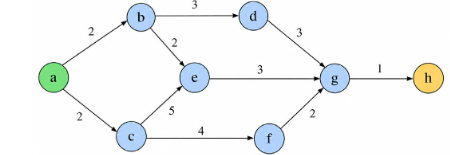
\includegraphics[width=0.95\linewidth]{../figures/graph_diagram.png}
\caption{Edge costs of the episodic shortest-path graph, identical to
Assignment 2.}
\label{fig:graph}
\end{figure}

\subsection{Neural Q-function}
The state is one-hot encoded (8-dim). The network has two hidden layers of
32 ReLU units and one linear output per action (7 actions total across all
states: $A_b,A_c,A_d,A_e,A_f,A_g,A_h$):
\begin{align}
h_1 &= \mathrm{ReLU}(W_1 s + b_1), \quad h_1\in\mathbb{R}^{32}\\
h_2 &= \mathrm{ReLU}(W_2 h_1 + b_2), \quad h_2\in\mathbb{R}^{32}\\
Q_\theta(s,\cdot) &= W_3 h_2 + b_3, \quad Q_\theta(s,\cdot)\in\mathbb{R}^{7}
\end{align}
Actions infeasible at the current state are masked by adding $+10^6$ to
their Q-value before any $\arg\min$ or $\min$ is taken -- the
cost-minimization analogue of $-\infty$ masking before a max. Trainable
parameters: $W_1{\in}\mathbb{R}^{32\times8}$ (256), $b_1$ (32),
$W_2{\in}\mathbb{R}^{32\times32}$ (1024), $b_2$ (32),
$W_3{\in}\mathbb{R}^{7\times32}$ (224), $b_3$ (7); \textbf{total
$1{,}575$} trainable parameters, counted directly from the instantiated
PyTorch module.

\subsection{Learning target and loss}
For a sampled transition $(s,a,c,s',d)$, with $d{=}1$ iff $s'{=}h$, the
target uses a separate target network $Q_{\theta^-}$:
\begin{equation}
y = c + \gamma(1-d)\min_{a'\in\mathcal{A}(s')} Q_{\theta^-}(s',a'),
\end{equation}
which reduces to $y=c$ at a terminal transition (no bootstrap). The online
network is trained by minibatch regression,
\begin{equation}
\mathcal{L}(\theta) = \frac{1}{B}\sum_{i=1}^{B}\big(y_i - Q_\theta(s_i,a_i)\big)^2,
\end{equation}
with $y_i$ detached from the autograd graph (semi-gradient: gradients flow
through the prediction $Q_\theta(s_i,a_i)$, never through $y_i$), using
Adam. \textbf{Experience replay} decorrelates consecutive gradient updates
-- every episode walks the same four-edge path, so training on transitions
in the order they occur would feed the optimizer a narrow, correlated
stream; sampling uniformly from a buffer breaks that correlation and reuses
past transitions. \textbf{The target network} is held fixed between hard
syncs so the regression target does not move on every gradient step the
prediction also moves on, which is what keeps the bootstrapped regression
from chasing itself.

\subsection{Training protocol}
Table~\ref{tab:hyper} lists the hyperparameters, all at the assignment's
suggested starting values, used unchanged for every seed. Each of the five
seeds (0--4) gets a freshly constructed online network, target network
(initialized equal to the online network), Adam optimizer, empty replay
buffer, and its own \texttt{numpy.random.Generator}, with
\texttt{random}, \texttt{numpy}, and \texttt{torch} global seeds reset to
the seed value; no seed continues training from another.

\begin{table}[t]
\centering
\caption{Hyperparameters (identical across all 5 seeds).}
\label{tab:hyper}
\footnotesize
\begin{tabular}{@{}ll@{}}
\toprule
Parameter & Value\\
\midrule
Hidden layers & 2 $\times$ 32, ReLU\\
Optimizer & Adam, lr $=10^{-3}$\\
Loss & MSE, Eq.~(5)\\
Replay capacity / warm-up & 10,000 / 200 transitions\\
Minibatch size & 32\\
Target update & hard copy every 100 opt. steps\\
Discount $\gamma$ & 1.0\\
Episodes per seed & 5000\\
$\epsilon$-greedy schedule & $1.00\to0.05$ linearly, episodes 1--4000; 0.05 after\\
Seeds & 0, 1, 2, 3, 4\\
\bottomrule
\end{tabular}
\end{table}

\section{Results and Evaluation}
\subsection{Training curves (seed 4)}
Fig.~\ref{fig:cost} shows seed 4's per-episode cost and its 100-episode
rolling mean. The raw cost takes only the values $\{8,9,10,11\}$ because
this graph has exactly four edges on every a-to-h path and the per-episode
cost is a sum of those discrete edge costs; the banding is a property of
the environment, not noise in the learner. The rolling mean drops from
about 9.2 early in training to settle near the $8.44$ reference line (the
Assignment-2 policy-iteration optimum) once $\epsilon$ reaches its $0.05$
floor around episode 4000, with the usual residual spread from that
exploration floor and the environment's own stochastic transitions.

\begin{figure}[t]
\centering
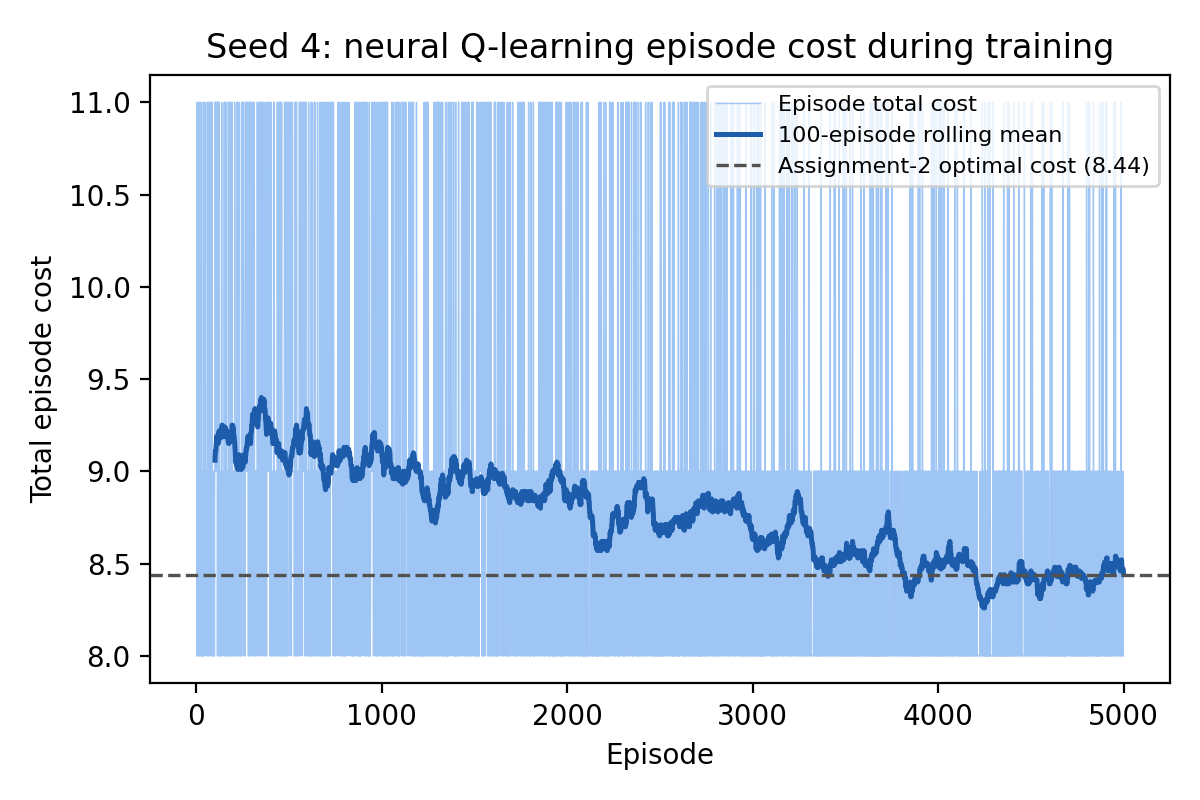
\includegraphics[width=\linewidth]{../figures/fig1_episode_cost_seed4.png}
\caption{Seed 4: per-episode total cost and its 100-episode rolling mean,
against the Assignment-2 optimal cost (dashed).}
\label{fig:cost}
\end{figure}

Fig.~\ref{fig:loss} plots the training loss (log scale) with a 200-step
rolling mean. The loss falls sharply over the first few hundred
optimization steps as the network leaves its random initialization, then
flattens to a noisy plateau around $0.1$--$0.2$ for the rest of training.
It does not fall toward zero, and we do not read that plateau as
convergence by itself: with $\epsilon$ never going below $0.05$ and the
environment's own $0.8/0.2$ randomness, even a network that exactly matched
the true optimal cost-to-go would still see nonzero squared error on every
minibatch, because the realized cost $c_i$ varies between samples of the
same $(s,a)$. The plateau is consistent with the network having reached a
stable estimate of the mean bootstrap target, not with the loss itself
vanishing.

\begin{figure}[t]
\centering
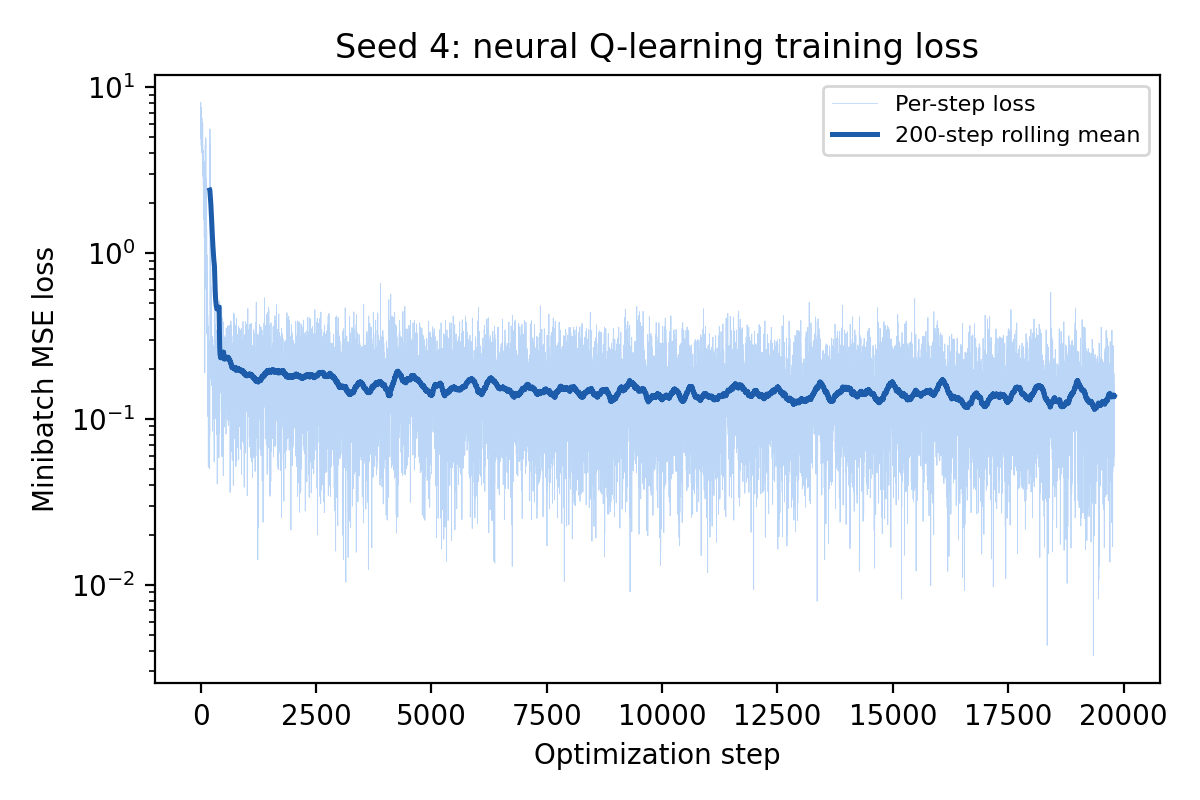
\includegraphics[width=\linewidth]{../figures/fig2_training_loss_seed4.png}
\caption{Seed 4: training loss (log scale) with a 200-step rolling mean.}
\label{fig:loss}
\end{figure}

\subsection{Learned policies and nominal paths}
All five independently trained networks (seeds 0--4) recovered the same
greedy policy at every one of the seven nonterminal states:
$\pi(a){=}A_b$, $\pi(b){=}A_e$, $\pi(c){=}A_f$, $\pi(d){=}A_g$,
$\pi(e){=}A_g$, $\pi(f){=}A_g$, $\pi(g){=}A_h$. This matches the optimal
policy from both policy iteration and tabular Q-learning in Assignment 2.
Under the intended transitions (the $0.8$-probability branch at every
decision), the nominal greedy path is $a\to b\to e\to g\to h$ for every
seed -- this is not the same as the expected stochastic path, since each
branching step still has a $0.2$ chance of landing on the alternate
successor.

\subsection{Stochastic evaluation (1000 episodes, $\epsilon=0$)}
Table~\ref{tab:eval} reports the frozen-network, exploration-off evaluation
for each seed, using an evaluation RNG stream (seeded at $100{,}000{+}$seed)
independent of the training RNG. Every seed reaches $h$ in $100\%$ of the
1000 episodes, with mean cost within $0.4\%$ of the $8.44$ optimum; the
spread between the per-seed means ($8.409$--$8.473$) is well inside one
standard deviation of a single seed's own evaluation noise ($\approx0.68$),
so it reads as sampling variability, not a meaningfully different learned
policy.

\begin{table}[t]
\centering
\caption{Five-seed stochastic evaluation, 1000 episodes/seed, $\epsilon=0$.}
\label{tab:eval}
\footnotesize
\begin{tabular}{@{}cccccc@{}}
\toprule
Seed & Mean & Std & Min & Max & \% reach $h$\\
\midrule
0 & 8.445 & 0.681 & 8.0 & 11.0 & 100.0\\
1 & 8.409 & 0.654 & 8.0 & 11.0 & 100.0\\
2 & 8.473 & 0.750 & 8.0 & 11.0 & 100.0\\
3 & 8.445 & 0.698 & 8.0 & 11.0 & 100.0\\
4 & 8.447 & 0.698 & 8.0 & 11.0 & 100.0\\
\midrule
PI optimal $V^*(a)$ & \multicolumn{5}{c}{8.440}\\
\bottomrule
\end{tabular}
\end{table}

\subsection{Hand verification}
We verified one real sampled transition against the trained seed-4
network: $(s{=}b, a{=}A_e)\to c{=}2, s'{=}e, d{=}0$. The online network
gives $Q_\theta(b,A_e){=}6.1291$; the target network (identical to the
online network at the end of training) gives
$\min_{a'}Q_{\theta^-}(e,a'){=}3.9649$ (the only feasible action at $e$ is
$A_g$, so the mask makes this exact). Substituting,
$y = 2 + 1.0(1-0)(3.9649) = 5.9649$, TD error $\delta = 5.9649 - 6.1291 =
-0.1642$, squared loss $\delta^2 = 0.0270$. Full forward-pass intermediate
values (all 32 hidden units), a separate hand-computed illustrative
2-hidden-unit example (explicitly not the trained weights), and a real
8-transition minibatch loss check are in \texttt{verification.md}.

\section{Discussion}
\subsection{Neural vs.\ tabular Q-learning}
Both methods see exactly the same thing during training: sampled
$(s,a,c,s',d)$ tuples, nothing more; neither ever touches
\texttt{TRANSITIONS} directly. Where they differ is what they do with
those samples. The tabular approach stores 10 Q-values, one per feasible
state-action pair (two actions each at $a,b,c$, one each at $d,e,f,g$),
and updates the corresponding entry after each transition. The network
uses 1,575 trainable parameters to approximate those same 10 values,
turning every transition into a gradient step through two ReLU layers --
a lot of extra machinery, on an 8-state problem, to represent something a
table already represents exactly.

Training stability tells a similar story. Assignment 2's tabular
Q-learning converged to the exact optimal policy, zero gap, on all 5
baseline seeds, with nothing beyond a learning rate and an
$\epsilon$-schedule. The network needed a target network and a replay
buffer just to keep the bootstrap target from chasing its own prediction,
and even with both in place the loss in Fig.~\ref{fig:loss} never goes
near zero; it plateaus around $0.1$--$0.2$ and stays noisy for the rest of
training. We do not read that as instability. The environment itself is
stochastic and $\epsilon$ never drops below $0.05$, so some irreducible
variance in the targets is expected. But it does mean that a decreasing
loss curve is not, by itself, evidence of convergence, which is the
caution the assignment asks us not to skip.

On outcomes the two methods land in the same place. All five neural
seeds recovered $a{\to}A_b$, $b{\to}A_e$, $c{\to}A_f$, matching tabular
Q-learning and policy iteration exactly, and the evaluation means in
Table~\ref{tab:eval} sit within about $\pm0.03$ of the $8.44$ optimum,
well inside a single seed's own evaluation noise -- a wash between the
two methods. The knob count is not: the table needs a learning rate and
an exploration schedule, full stop; the network needs those plus an
architecture, an optimizer and its learning rate, a replay capacity and
warm-up length, a batch size, and a target-update period. Training all
five neural seeds took about 30 seconds each on CPU ($\approx$19,800
gradient steps per seed); the tabular baseline from Assignment 2 finishes
in a fraction of that, with no PyTorch, no autograd graph, and no tensor
overhead for what amounts to 10 scalar Q-values.

\subsection{Is neural Q-learning beneficial here?}
No, not for this problem. Eight states and seven actions fit a Q-table
trivially, and tabular Q-learning already reaches the exact optimum with
less code, no architecture choice, and less compute. The network
reproduces the same answer -- a useful sanity check that the
implementation is correct -- but it adds real complexity (replay buffer,
target network, masking, extra hyperparameters) that buys nothing here.
The case for a neural Q-function is the one Lecture 9 makes: states that
cannot be enumerated or stored in a table at all, not a problem that
already fits in one.

\section{Conclusion}
A small feedforward network trained with replay and a target network, on
sampled transitions only, recovered the exact tabular-optimal policy and
cost on this 8-state problem across all 5 independent seeds -- good
evidence the DQN-style update is implemented correctly. The main
limitation is scale: an 8-state, 1575-parameter problem can't show what
function approximation is actually for (generalizing across large or
continuous state spaces), so nothing here says neural Q-learning scales
well, only that on this particular small problem it reaches the same
place tabular Q-learning does, at higher cost.

\section*{README / Reproducibility}
\textbf{Software:} Python 3.13.9, PyTorch 2.15.0 (CPU build), NumPy 2.4.2,
Matplotlib 3.10.8. \textbf{Hardware:} Windows 11, CPU-only, no GPU.
\textbf{To run:} \texttt{cd code \&\& python neural\_q\_learning.py} trains
all 5 seeds ($\approx$30 s/seed) and writes \texttt{results/} and
\texttt{figures/}; \texttt{python hand\_verification.py} regenerates the
Section~III-D numbers. Code and full results:
\url{https://github.com/Chinmay-Prashanth/eee598-neural-q-learning}.

\section*{AI Assistance Disclosure}
The team developed the solution, performed the experiments, and analyzed
the results independently. Generative AI tools were used to assist with
code optimization and to improve the vocabulary, grammar, and readability
of the report. The final implementation and results were reviewed and
verified by the team.

\end{document}
